\documentclass[11pt]{article}

\usepackage[margin=1in]{geometry}
\usepackage{amsmath,amssymb,mathtools}
\usepackage{enumitem}
\usepackage{xurl}
\usepackage{import}
\usepackage{tabularx}
\usepackage{array}
\usepackage{longtable}
\usepackage{float}
\usepackage{microtype}
\usepackage{graphicx}

\usepackage{tikz}
\usetikzlibrary{positioning,arrows.meta,decorations.pathmorphing}

\usepackage{pgfplots}
\pgfplotsset{compat=1.18}

\usepackage{titlesec}
\setcounter{secnumdepth}{3}
\setcounter{tocdepth}{2}

\usepackage[
    backend=biber,
    style=numeric,
    sorting=none
]{biblatex}
\addbibresource{bib.bib}

\usepackage{hyperref}
\hypersetup{
    colorlinks=true,
    linkcolor=blue, % sections, figures, tables, equations, contents
    citecolor=blue, % citations
    urlcolor=blue,  % URLs
    pdftitle={Physical Biology of the Cell: Conceptual Notes},
    pdfauthor={Chinmayi Subramanya}
}

\newcommand{\cs}[1]{\textcolor{blue}{#1}}

\titleformat{\paragraph}
{\normalfont\normalsize\bfseries}{\theparagraph}{1em}{}
\titlespacing*{\paragraph}
{0pt}{3.25ex plus 1ex minus .2ex}{1.5ex plus .2ex}


\newcommand{\dd}{\mathrm{d}}
\newcommand{\Dt}{\Delta t}

% ------------------------------------------------------------
% Mini plots for distributions
% ------------------------------------------------------------
% ------------------------------------------------------------
% Mini plots for probability distributions
% ------------------------------------------------------------

\newcommand{\miniBinomial}{%
    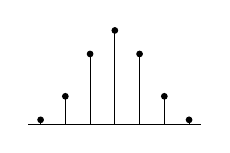
\begin{tikzpicture}[baseline=(current bounding box.center)]
        \begin{axis}[
            width=2.2cm,
            height=1.3cm,
            scale only axis,
            axis x line*=bottom,
            axis y line=none,
            xtick=\empty,
            ytick=\empty,
            xmin=-0.5,
            xmax=6.5,
            ymin=0,
            ymax=0.34
        ]
            \addplot[ycomb,mark=*,mark size=1pt] coordinates {
                (0,0.0156)
                (1,0.0938)
                (2,0.2344)
                (3,0.3125)
                (4,0.2344)
                (5,0.0938)
                (6,0.0156)
            };
        \end{axis}
    \end{tikzpicture}%
}

\newcommand{\miniPoisson}{%
    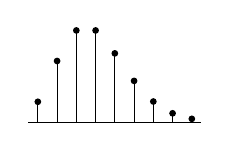
\begin{tikzpicture}[baseline=(current bounding box.center)]
        \begin{axis}[
            width=2.2cm,
            height=1.3cm,
            scale only axis,
            axis x line*=bottom,
            axis y line=none,
            xtick=\empty,
            ytick=\empty,
            xmin=-0.5,
            xmax=8.5,
            ymin=0,
            ymax=0.25
        ]
            \addplot[ycomb,mark=*,mark size=1pt] coordinates {
                (0,0.0498)
                (1,0.1494)
                (2,0.2240)
                (3,0.2240)
                (4,0.1680)
                (5,0.1008)
                (6,0.0504)
                (7,0.0216)
                (8,0.0081)
            };
        \end{axis}
    \end{tikzpicture}%
}

\newcommand{\miniGaussian}{%
    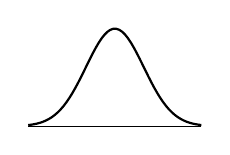
\begin{tikzpicture}[baseline=(current bounding box.center)]
        \begin{axis}[
            width=2.2cm,
            height=1.3cm,
            scale only axis,
            axis x line*=bottom,
            axis y line=none,
            xtick=\empty,
            ytick=\empty,
            xmin=-3,
            xmax=3,
            ymin=0,
            ymax=1.05,
            domain=-3:3,
            samples=60
        ]
            \addplot[thick] {exp(-x^2/2)};
        \end{axis}
    \end{tikzpicture}%
}

\newcommand{\miniExponential}{%
    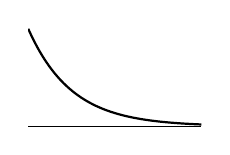
\begin{tikzpicture}[baseline=(current bounding box.center)]
        \begin{axis}[
            width=2.2cm,
            height=1.3cm,
            scale only axis,
            axis x line*=bottom,
            axis y line=none,
            xtick=\empty,
            ytick=\empty,
            xmin=0,
            xmax=4,
            ymin=0,
            ymax=1.05,
            domain=0:4,
            samples=60
        ]
            \addplot[thick] {exp(-x)};
        \end{axis}
    \end{tikzpicture}%
}

\newcommand{\miniGeometric}{%
    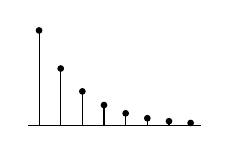
\begin{tikzpicture}[baseline=(current bounding box.center)]
        \begin{axis}[
            width=2.2cm,
            height=1.3cm,
            scale only axis,
            axis x line*=bottom,
            axis y line=none,
            xtick=\empty,
            ytick=\empty,
            xmin=-0.5,
            xmax=7.5,
            ymin=0,
            ymax=0.43
        ]
            \addplot[ycomb,mark=*,mark size=1pt] coordinates {
                (0,0.4000)
                (1,0.2400)
                (2,0.1440)
                (3,0.0864)
                (4,0.0518)
                (5,0.0311)
                (6,0.0187)
                (7,0.0112)
            };
        \end{axis}
    \end{tikzpicture}%
}

\title{\huge{Physical Biology of the Cell} \\ \medskip 
\Large{Rob Phillips and Jan\'{e} Kondev} \\ \medskip
\large{MPI CBG, Dresden}
}
\date{October 5-9, 2026}
\author{Course Notes by Chinmayi Subramanya}
\newcommand{\conceptualedition}{Conceptually organized edition}


\begin{document}
\maketitle
% \begin{center}\conceptualedition\end{center}
\paragraph*{How to read these notes}
The main text follows a conceptual progression from quantities and rate models to probability, diffusion, statistical mechanics, and useful representations.
The appendices provide mathematical tools, detailed derivations, reading lists, the original daily sequence, and notation.
% The source files distinguish added navigation and conceptual bridges with \texttt{EDITORIAL ADDITION} comments.
% The original day-by-day files are retained separately in the project for reference.

\paragraph*{Mathematical methods reference}
Appendix~\ref{app:math} is a working reference for readers who have not previously encountered all the mathematical methods used in these notes.
It focuses on how to read the notation, what the mathematical objects represent, how to calculate with them, and when each method is useful.
The appendix is not intended to be read linearly before the main text.
When a mathematical step becomes unfamiliar, consult the corresponding topic below.

\begin{center}
\begin{tabularx}{\textwidth}{@{}>{\raggedleft\arraybackslash}p{2em}>{\raggedright\arraybackslash}X>{\raggedright\arraybackslash}p{0.25\textwidth}@{}}
& \textbf{Concept} & \textbf{Section to consult} \\
\hline
1. & Reading notation, exponentials, logarithms, units, and scales & Sections~\ref{math:language} and~\ref{sec:scale} \\
2. & Derivatives, integrals, partial derivatives, and conservation & Section~\ref{math:calculus} \\
3. & Taylor expansions and interpolation between known points & Sections~\ref{math:taylor}-\ref{math:interpolation} \\
4. & ODEs, master equations, PDEs, and time evolution & Sections~\ref{math:ode}-\ref{math:separation} \\
% \ref{math:master}, and 
5. & Vectors, matrices, eigenvectors, and eigenfunctions & Sections~\ref{math:linear}-\ref{math:eigen} \\
6. & Fourier series, spatial modes, and delta distributions & Section~\ref{math:fourier} \\
7. & Probability, expectation, variance, and waiting times & Sections~\ref{math:probability}-\ref{math:survival} \\
8. & Counting states, Boltzmann weights, free energy, and entropy & Sections~\ref{math:combinatorics}-\ref{math:constraints} \\
9. & Least squares, covariance, correlation, and PCA & Sections~\ref{math:least-squares}-\ref{math:pca} \\
\hline
\end{tabularx}
\end{center}

\medskip
\paragraph*{Acknowledgements}
These notes were compiled from notes typed during the course, with the assistance of OpenAI's GPT-5.6 Sol for transcription, organization, and editing. The material has been reorganized thematically rather than following the chronological sequence of the lectures. Any errors or omissions are my own.

\clearpage

\tableofcontents

\import{sections/}{01-life.tex}
\import{sections/}{02-rates.tex}
\import{sections/}{03-probability.tex}
\import{sections/}{04-diffusion.tex}
\import{sections/}{05-states.tex}
\import{sections/}{06-representations.tex}
\import{sections/}{07-philosophy.tex}

\newpage 
\appendix
\import{appendix/}{appendix-a-math.tex}
\import{appendix/}{appendix-b-derivations.tex}
\import{appendix/}{appendix-c-readings.tex}
\import{appendix/}{appendix-d-daily-flow.tex}
\import{appendix/}{appendix-e-notation.tex}

\clearpage
\printbibliography[heading=bibintoc,title={References}]

\end{document}
